%%
%% 研究報告用スイッチ
%% [techrep]
%%
%% 欧文表記無しのスイッチ(etitle,eabstractは任意)
%% [noauthor]
%%

%\documentclass[submit,techrep]{ipsj}
\documentclass[submit,techrep,noauthor]{ipsj}



\usepackage[dvipdfmx]{graphicx}
\usepackage{latexsym}

\def\Underline{\setbox0\hbox\bgroup\let\\\endUnderline}
\def\endUnderline{\vphantom{y}\egroup\smash{\underline{\box0}}\\}
\def\|{\verb|}
%

%\setcounter{巻数}{59}%vol59=2018
%\setcounter{号数}{10}
%\setcounter{page}{1}


\begin{document}


\title{GPS・QZSSを使用した自動走行}

\etitle{Autonomous Driving Utilizing GPS and QZSS}

\affiliate{NKHS}{日本工学院北海道専門学校\\
Nihon Kogakuin Hokkaido College}

\author{大川 倫典}{Okawa Michinori}{NKHS}
\author{高谷 健汰}{Takaya Kenta}{NKHS}
\author{山家 裕樹}{Yamaga Yuki}{NKHS}

\begin{abstract}
本稿は,GPS・QZSSを使用したラジコンカーの自動走行の研究についてまとめたものである.\\
Raspberry Piとジャイロセンサ,GPS受信機を用いてラジコンカーを制御し座標と旋回角度による自動走行を実現する.\\
 本研究は,例年10月に開催されている\textbf{「GPS・QZSSロボットカーコンテスト」}での入賞を目標としている.昨年度から実装に取り掛かっており,現在は座標を利用した区間の切り替えの調整を行っている.

\end{abstract}

%
%\begin{jkeyword}
%情報処理学会論文誌ジャーナル,\LaTeX,スタイルファイル,べからず集
%\end{jkeyword}
%
%\begin{eabstract}
%This document is a guide to prepare a draft for submitting to IPSJ
%Journal, and the final camera-ready manuscript of a paper to appear in
%IPSJ Journal, using {\LaTeX} and special style files.  Since this
%document itself is produced with the style files, it will help you to
%refer its source file which is distributed with the style files.
%\end{eabstract}
%
%\begin{ekeyword}
%IPSJ Journal, \LaTeX, style files, ``Dos and Dont's'' list
%\end{ekeyword}

\maketitle
%1
\section{研究概要}

%1.1
\subsection{テーマ決定の理由}
IoTを主とした研究に取り組みたいと考えていた中で,GPSを用いたロボットカーのコンテストが開催されていることを知った.コンテストに挑戦することで技術力の向上につながると感じ,研究テーマとした.


%1.2
\subsection{研究概要}
本研究は,例年秋に開催されている「GNSS・QZSSロボットカーコンテスト」での入賞を目指すことで,技術力を向上させることを目標としている.コンテスト終了後は校内のサーキットコースでの走行とUIでの走行が可能なアプリケーションの開発を検討している.




%2
\section{環境}


%2.1
\subsection{使用機器}
この研究で使用する機器は以下のとおりである.

\begin{enumerate}
\item \|TAMIYA Rock Socker CR-01|: 走行体
\item \|TBLE-04S      |: スピードコントローラー
\item \|AO-5052 TSU-03サーボ |: サーボモータ
\item \|Raspberry Pi4 ModelB|: シングルボードコンピュータ
\item \|Raspberry Pi Sence HAT |: ジャイロセンサ
\item \|ZED-F9P |: GNSSモジュール
\item \|NEO-D9C |: CLASモジュール
\item \|BT-345AJL2 |: GNSS受信機
\end{enumerate}


%2.2
\subsection{開発環境}
開発環境は以下のとおりである.
\begin{enumerate}
\item \|Python| : 開発言語 
\item \|Raspberry Pi OS 11| : OS %後でバージョンまで書く 
\end{enumerate}


%2.3
\subsection{システム構成図}
システムの構成図を図1に,その凡例を図2に示す.

\begin{figure}[h]
 \centering
   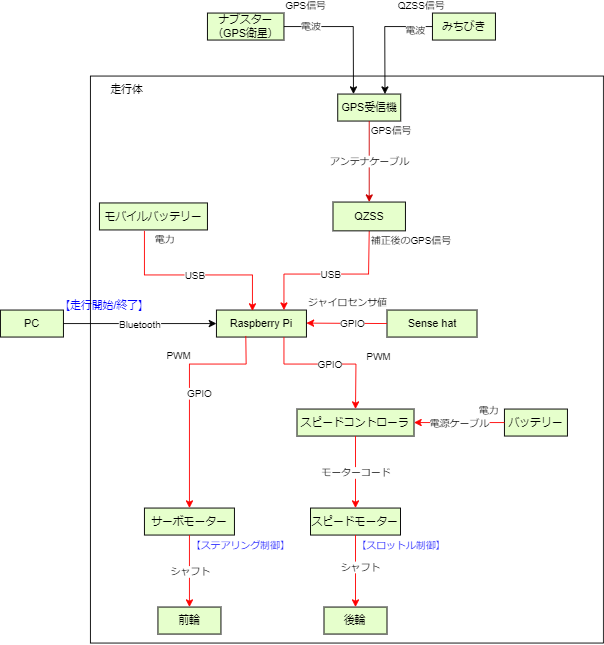
\includegraphics[scale=0.38]{Sys.png}
 \caption{システム構成図}
 \label{システム構成図}
\end{figure}

\begin{figure}[h]
 \centering
   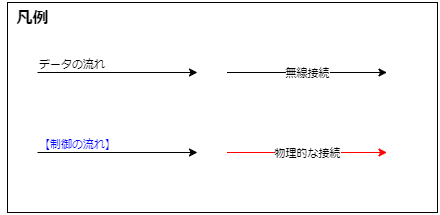
\includegraphics[scale=0.25]{hanrei.png}
   \caption{システム構成図の凡例}
 \label{システム構成図の凡例}
\end{figure}


%ここにシステム構成の留意点を説明する

\newpage

\subsection{パッケージ図}
走行システムのパッケージ図を図3に示す

\begin{figure}[h]
 \centering
   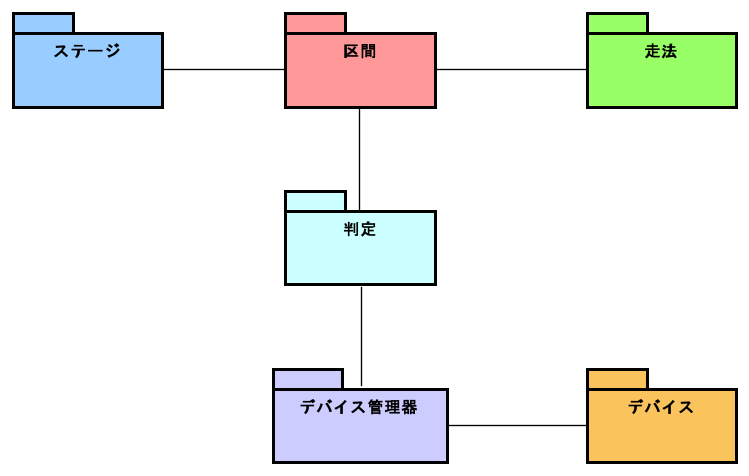
\includegraphics[scale=0.37]{package.png}
 \caption{走行システムのパッケージ図}
 \label{パッケージ図}
\end{figure} 

%パッケージについて軽く説明を入れる


%3
\section{GPS・QZSSについて}

\subsection{GPSとは}
Global Positioning Systemの略で,アメリカ合衆国によって運営されている衛星測位システムである.
上空の衛星から信号を受け取ることで現在位置や時刻を計算することができる.\\
 数メートルの誤差は出てしまうが世界中どこでも受信することができ,カーナビやスマートフォンなど身近なものにも使用されている技術である.


\subsection{QZSSとは}
Quasi-Zenith Satellite Systemの略で,日本及びアジア太平洋地域向けの衛星システムである.同じ衛星システムとしてGPSがよく知られていることから「日本版GPS」と呼ばれることもある.\\
 準天頂衛星「みちびき」からGPSよりも局地的な位置情報を取得でき,GPSの誤差をセンチメートル単位まで補正する「CLAS(Centimeter Level Augmentation Service)」を利用することができる.

\section{GPS・QZSSロボットカーコンテスト}
\subsection{大会概要}
学生の衛星測位技術に関する基礎技術を修得及び技術者の交流を目的として開催されるコンテストである.\\
 走行体にGPS受信機を搭載して自律的に走行させ、獲得したポイントを競う大会.
 GNSS受信機以外にジャイロセンサー・地磁気センサーのみ使用可能となっている.\\
 大会レギュレーションはオンラインのみでの参加など3つのカテゴリーに分かれているが,私たちはカテゴリー1の会場での参加を目指している.
 
 \subsection{開催日程}
 開催日程の詳細を以下に示す.
 
 10月22日(日) 10:00~15:00\\
 東京海洋大学  越中島キャンパス

%ここに開催日時と開催場所を記入する

\subsection{競技ルール}
競技コースの概要を図4に示す.



\begin{figure}[h]
 \centering
   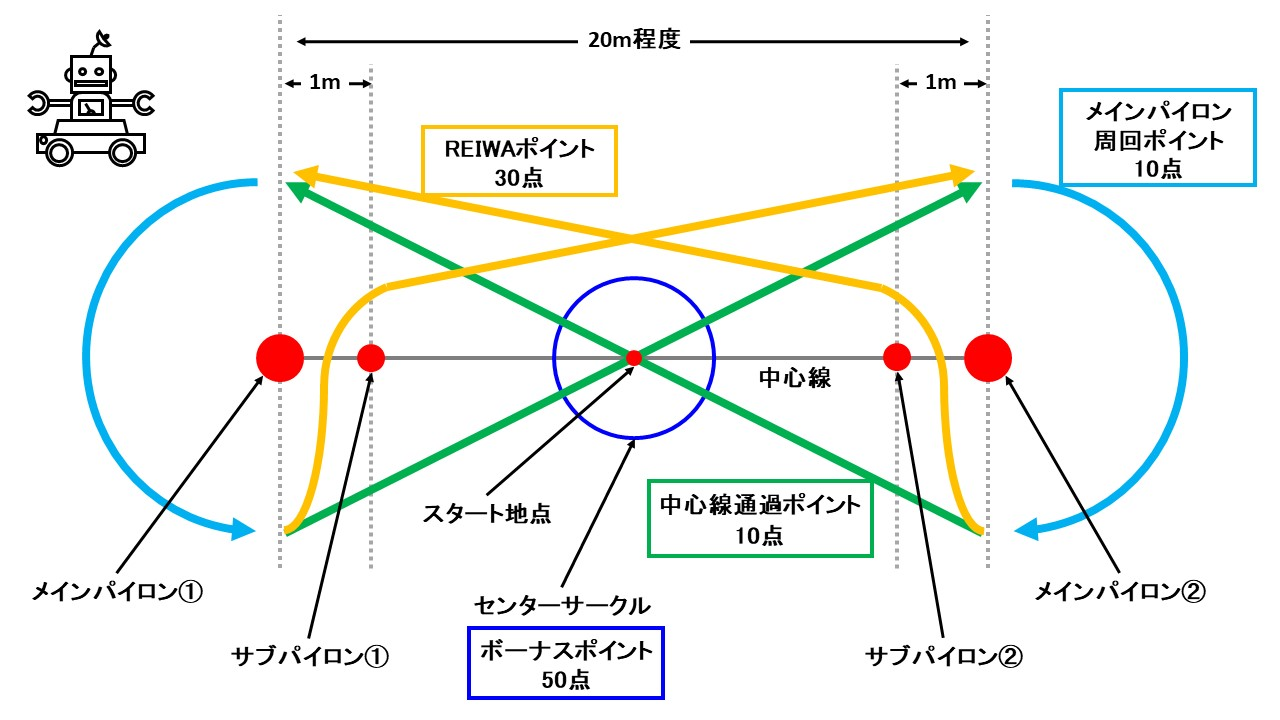
\includegraphics[scale=0.23]{rules.jpg}
 \caption{競技コース}
 \label{大会ルール}
\end{figure}

競技コース上を8の字に走行し,特定の条件を満たすことでポイントを獲得できる.ポイントの詳細を表1に示す.
 
 \begin{center}

 
 \begin{table}[h]
  \caption{ポイント詳細}
  \label{ラベル名}
  \centering
  
  \begin{tabular}{|c|r|l|}
  \hline
    ポイント名 & 加点 & 条件 \\
    \hline 
    
    \begin{tabular}{c}
    メインパイロン\\周回ポイント
   
    \end{tabular} & 10 & メインパイロンを半周する \\
    
    \hline
    
    \begin{tabular}{c}
    中心線\\通過ポイント
   
    \end{tabular}& 10 & 
    \begin{tabular}{l}
    メインパイロンを半周した後\\メインパイロン間を\\結ぶ中心線を通過する
    \end{tabular}\\
    \hline
    
    REIWAポイント & 30 & 
    \begin{tabular}{l}
    メインパイロンを半周した後\\そのメインパイロンとセットとなる\\サブパイロンとの間を通過する
    \end{tabular}\\
    \hline
    
    ボーナスポイント & 50 & 
    \begin{tabular}{l}
    メインパイロン周回ポイントを\\獲得した上で競技時間内に\\センターサークル内に停止する
    \end{tabular}\\
    \hline
    
    救済措置 & -5 & 
    \begin{tabular}{l}
    障害物を動かす,または\\走行体の向きを変える\\
    競技中に5回まで行うことが出来る
    \end{tabular}\\
    \hline
    
    \end{tabular}
\end{table}

\end{center}

また,競技中に走行体が進行不能となった場合にリトライを宣言することが出来る.
リトライが主審に許可された場合,走行体の位置や向きを再調整後に再度走行を開始できる.
しかし今まで獲得したポイントは0になり,経過した競技時間はリセットされないため注意が必要となる.

\subsection{大会結果}

\section{走行アルゴリズム}
\subsection{仮想ライントレース}7
私たちは現在,座標で設定された目標地点まで直進し到達した時点で走行を停止する段階まで実装し,動作を確認している.
仮想ライントレースという仕組みを用いて走行している.
仮想ライントレースのイメージ図を図5に示す.

\begin{figure}[h]
 \centering
   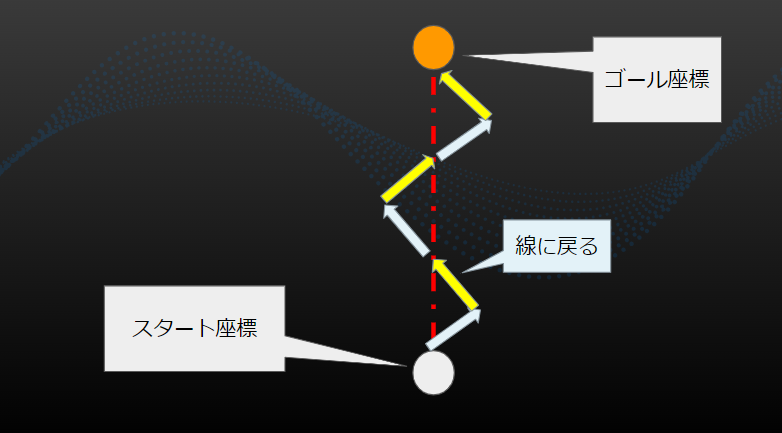
\includegraphics[scale=0.48]{vr_line.png}
 \caption{仮想ライントレースのイメージ図}
 \label{仮想ライントレースのイメージ図}
\end{figure}

開始地点から目標地点まで仮想上の線を引き,その上を走行することで目標地点にたどり着く手法である.\\
直進と旋回でそれぞれアルゴリズムが異なる.\\

\subsubsection{直線仮想ライントレース}
現在地と目標地点の2点を仮想上の直線で結び、ライン上を走行する.\\

直線仮想ライントレースのイメージ図を図6に示す.\\

\begin{figure}[h]
 \centering
   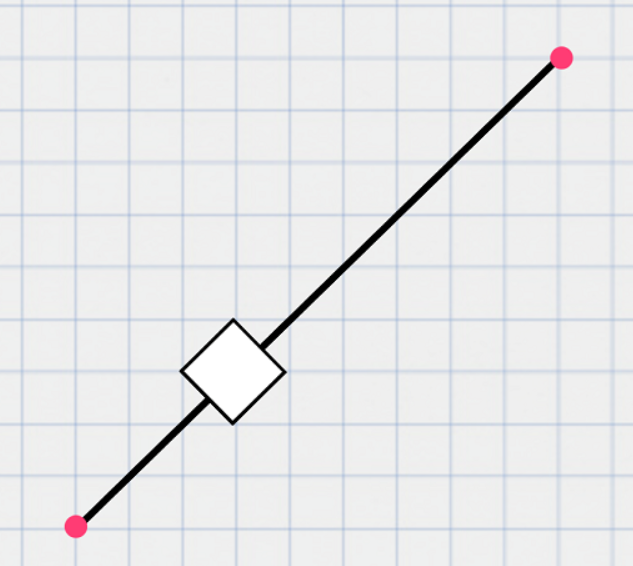
\includegraphics[scale=0.4]{LineTrace.png}
 \caption{直線仮想ライントレースのイメージ図}
 \label{直線仮想ライントレースのイメージ図}
\end{figure}


\subsubsection{曲線仮想ライントレース}
2点間の中点と現在地を直線で結び,その長さが変わらないように旋回することで目標地点にたどり着く.\\
曲線仮想ライントレースのイメージ図を図7に示す.\\
\begin{figure}[h]
 \centering
   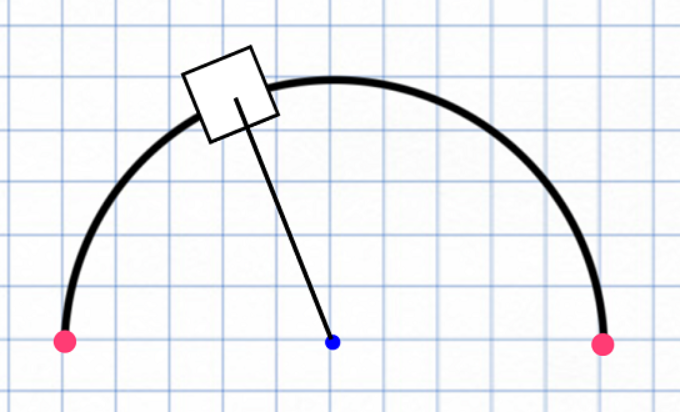
\includegraphics[scale=0.48]{curveLineTrace.png}
 \caption{曲線仮想ライントレースのイメージ図}
 \label{曲線仮想ライントレースのイメージ図}
\end{figure}

\subsection{PID制御}
目標値に対して大小を比較し操作を決定する制御を「オンオフ制御」の実装でもライントレースは可能だが,ラインを通り過ぎてしまう.オンオフ制御の欠点を補うために「PID制御」を実装する.
PID制御は目標値周辺で操作量を変化させ,
\subsection{座標変換}
GPS受信機で受信しているGPS信号は,地球を球体として緯度・経度で表現されている「地理座標系」というものである.\\
私たちが作成しているプログラムは平面を想定しており,地理座標系のままでは正確な距離や角度を算出することができない.
そのため地理座標系から「平面直角座標系」への変換を行う必要がある.\\
座標の変換にはpyprojというライブラリを使用している.\\
座標変換のイメージ図を図6に示す.

\begin{figure}[h]
 \centering
   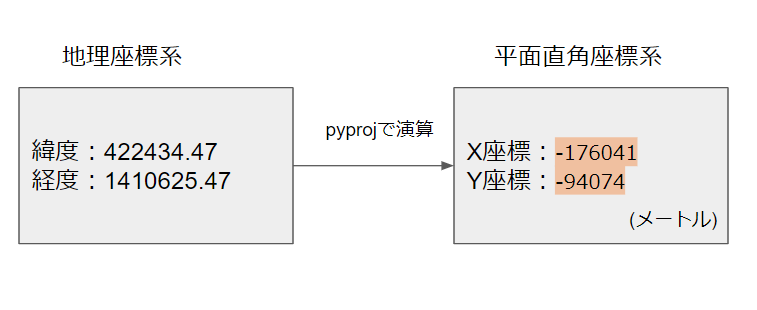
\includegraphics[scale=0.48]{GPS2xy.png}
 \caption{座標変換のイメージ図}
 \label{仮想ライントレースのイメージ図}
\end{figure}

平面直角座標系は地域によって19の系番号が割り振られており,原点が分かれている.\\
登別市や室蘭市は系番号12となる.座標の原点を図7に示す.\\

\begin{figure}[h]
 \centering
   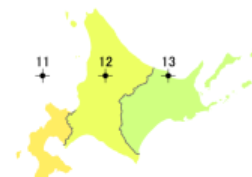
\includegraphics[scale=1.0]{origin.png}
 \caption{平面直角座標系の原点}
 \label{origin}
\end{figure}



\subsection{サーキットコースでの走行}
コンテストが終わってからの実装を予定しているため,現時点では未実装となっている.
コンテストが終わり次第実装を初め,11月下旬までに実装を完了する予定である.


%サーキットコースでの走行について,またGUIの作成は断念する方向で行くことも触れるかもしれない.
  

% 同一の走法で走行できるエリアを一つの区間として扱い,区間を切り替えることで走法や走行速度などのパラメータを変更している.\\
%直進時は「直線仮想ライントレース」,旋回時は「曲線仮想ライントレース」という二つの走法を使って走行する.\\
%「判定」には区間を切り替えるために座標等の条件から判定をし論理型を返す.\\

\label{config}



%4.1.2



%6
\section{おわりに}
設定された目標座標に向かって直進することはできているが,ON/OFF制御での実装であり走行精度が望ましくないため,早急にPID制御の実装を完成させる必要がある.そのうえ旋回部分を担う「曲線仮想ライントレース」の実装が完了していないため,この2つの実装を早急に完成させた後,コンテスト優勝に向けた戦略を練りシステムを改善していきたい.


\end{document}
